\exercise{Zooming and shrinking by bilinear interpolation}
\subsection*{a - \texttt{IPresizebl}}
For this exercise, a \textit{MATLAB} function was made that is able to rescale an image.
The pixels of the rescaled image have to be interpolated in the original image, using bilinear interpolation.
This means that we look at the four pixels in the original image that are closest to the required position, and take the weighted average of those.

The code is given and explained below:
\matlabexternal{IPresizebl.m}

\subsection*{a - Resizing a chronometer}
The file \texttt{chronometer1250dpi.tif} is an image file of a very high resolution.
For some purposes it is useful to have a smaller images.
Our function, \texttt{IPresizebl} is made for exactly this purpose (among others).

The original image is shown in Figure \ref{fig:tiger}

\begin{figure}
\centering
\begin{subfigure}[b]{0.4\textwidth}
\includegraphics[width=\textwidth]{originalChrono.eps}
\caption{A tiger}
\label{fig:tiger}
\end{subfigure}
~
\begin{subfigure}[b]{0.4\textwidth}
\includegraphics[width=\textwidth]{rescaledUpChrono.eps}
\caption{A mouse}
\label{fig:mouse}
\end{subfigure}
\caption{Pictures of animals}\label{fig:animals}
\end{figure}

\begin{figure}
 \centering
 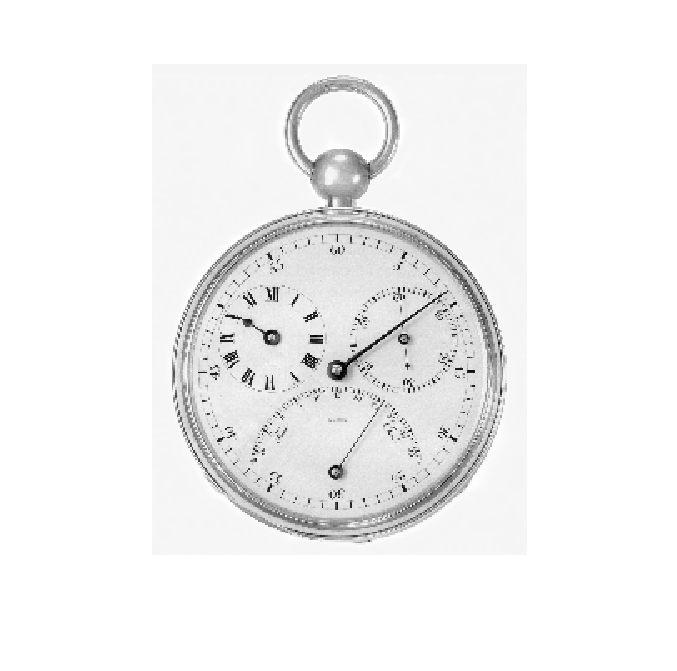
\includegraphics{scaledDownChrono.eps}
 \caption{Downscaled chromometer}
 \label{fig:chromo_down}
\end{figure}